\documentclass[aps,prb,twocolumn,letterpaper,twoside,nobalancelastpage,groupedaddress,amsmath,amssymb,floatfix,citeautoscript]{revtex4-1}
%\usepackage{geometry}       
%\geometry{letterpaper}     
%\usepackage[parfill]{parskip}    % Activate to begin paragraphs with an empty line rather than an indent
\usepackage{graphicx}
\usepackage{bm} %bold math symbols
\usepackage{times}
\usepackage{graphicx}
\usepackage{physics}
\usepackage{outlines}             
\usepackage{amssymb}
\usepackage[caption=false]{subfig}
\usepackage{mathtools}
\usepackage{color}
\definecolor{darkred}{rgb}{0.6,0.,0.}
\definecolor{darkgreen}{rgb}{0.,0.5,0.}
\definecolor{darkblue}{rgb}{0.,0.,0.6}

\usepackage{framed}

%\usepackage[square,numbers,sort,merge]{natbib}
\usepackage[
breaklinks,
colorlinks=true,
linkcolor=darkred,
citecolor=darkgreen,
urlcolor=darkblue]{hyperref}
%\usepackage{doi}

% \DeclareMathOperator{\tr}{tr}
% \DeclareMathOperator{\erf}{Erf}

\DeclareGraphicsRule{.tif}{png}{.png}{`convert #1 `dirname #1`/`basename #1 .tif`.png}

\begin{document}


\def \Ns {\mathbb{N}}
\def \Rs {\mathbb{R}}
\def \Zs {\mathbb{Z}}
\def \Qs {\mathbb{Q}}
\def \Cs {\mathbb{C}}
\def \id {\mathbb{I}}

\def \bfq {{\bf q}}
\def \bfp {{\bf p}}
\def \bfx {{\bf x}}
\def \bfy {{\bf y}}
\def \bfz {{\bf z}}
\def \bfr {{\bf r}}
\def \bfk {{\bf k}}
\def \bfn {{\bf n}}
\def \bfb {{\bf b}}
\def \bfm {\mathbf{m}}
\def \bfn {\mathbf{n}}

%\def \hata {{a}}
%\def \hatadag {{a}^{\dagger}}

\def \hatq {\widehat{q}}
\def \hatp {\widehat{p}}
\def \hata {\widehat{a}}
\def \hatadag {\widehat{a}^{\dagger}}
%\def \hatb {\widehat{b}^\phantom{\dagger}}
%\def \hatbdag {\widehat{b}^{\dagger}}
\def \wtN {\widetilde{N}}

\def \ve {\varepsilon}
\def \vth {\vartheta}



\title{Non-Landau level cyclotron orbits and the quantum Hall effect in Harper-Hofstadter bands}
\author{David Bauer}
\email{dbauer@physics.ucla.edu}
\affiliation{Department of Physics and Astronomy, University of California at Los Angeles, 475 Portola Plaza, Los Angeles, California 90095, USA}

\author{Fenner Harper}
\affiliation{Department of Physics and Astronomy, University of California at Los Angeles, 475 Portola Plaza, Los Angeles, California 90095, USA}

\author{Rahul Roy}
\affiliation{Department of Physics and Astronomy, University of California at Los Angeles, 475 Portola Plaza, Los Angeles, California 90095, USA}

\date{\today}
\begin{abstract}
Recent developments in fractional quantum Hall (FQH) physics suggest the importance of studying FQH phases of particles occupying single-particle states that are not Landau levels. FQH phases in the regime of strong lattice effects, called fractional Chern insulators (FCI), provide one setting for such studies. As the stength of lattice effects vanishes, the bands of generic lattice models asymptotically approach Landau levels. In this article, we construct non-generic lattice models for single-particle bands that are distinct from Landau levels even in this asymptotic limit. In particular, we study a finely-tuned model with effective continuum hamiltonian with purely quartic dependence on momentum. We describe how the distinction between such bands and Landau levels may be quantified by magnetic Brillouin zone (MBZ) geometry, and we compare the stability of FQH phases in various regimes.
\end{abstract}

% \pacs{0}

\maketitle

\section{Introduction}
The incompressible liquid phases of the fractional quantum Hall effect (FQHE) serve as prototypical examples of topologically ordered or gapped quantum liquid phases\cite{yoshioka_quantum_2002,fradkin_field_2013} in 2+1 dimensions. These phases are characterized by their long-range entanglement structure, which gives rise to topological quasiparticles and universal, quantized linear responses. Theoretical models of the quantum Hall (QH) fluid -- based, for example, on model wavefunctions \cite{laughlin_anomalous_1983} -- often make the simplifying assumption that the microscopic constitutent particles occupy states in a single Landau level. Some properties of Landau levels, such as nonzero Chern number \cite{thouless_quantized_1982}, are essential for the QHE, but recent work points to a need to understand the QHE in the case that the single-particle states are not Landau levels.

Among such work is the observation, due to Haldane, that the FQH fluid carries an emergent geometrical degree of freedom\cite{haldane_geometrical_2011} corresponding to the shape of elementary composite particles or `droplets.' \cite{johri_probing_2016} The geometry of the FQH fluid manifests in part through universal contributions to linear responses corresponding to perturbative variations in geometry, of which the Hall viscosity\cite{avron_viscosity_1995,tokatly_lorentz_2007,read_non-abelian_2009,haldane_hall_2009} is an example. In topological fluids, the Hall viscosity has a universal part proportional to the topological spin of the fluid\cite{read_non-abelian_2009}, which is related to the composite droplet shape.\cite{johri_probing_2016} This geometrical degree of freedom may be obscured by the introduction of non-generic symmetries to the FQH problem implicitly, via the assumption that the underlying single-particle bands are Landau levels.

The study of the FQH beyond Landau levels has also been spurred by the discovery of fractional Chern insulators (FCI) -- time-reversal (TR) symmetry-breaking, fractionalized phases observed in the regime of strong lattice effects \cite{Bergholtz:2013ue,parameswaran_fractional_2013}. In this regime, the single-particle states reside in Chern bands rather than Landau levels. The addition of a non-negligible lattice potential introduces additional geometric data that may break some non-generic symmetries. For example, in the case of a square lattice, $SO(2)$ rotational invariance in the coordinate plane is explicitly broken to $C_4$ lattice symmetry. From this point of view, a complete theory of the FQHE formulated as generically as possible should furnish a theory of FCI phases. Understanding how the lattice potential of FCIs affects the geometrical responses of their topological fluid states is an active research subject. \cite{shapourian_viscoelastic_2015}

 In this article, we study the geometry of Chern bands over the magnetic Brillouin zone (MBZ) parameterizing eigenstates of magnetic translations operators\cite{zak_magnetic_1964}. While this geometry is distinct from the emergent, many-body geometry of the FQH fluid, studies of FCIs have described how single-particle geometry influences the stability of many-body FQH phases through the GMP/$w_{\infty}$ algebra of band-projected density operators.\cite{Girvin:1986bu,parameswaran_fractional_2012,parameswaran_fractional_2013, roy_band_2014} This connection is substantiated by numerical studies \cite{jackson_geometric_2015,Claassen2015,bauer_quantum_2016}, and researchers have employed it to engineer `ideally' stable FCI models \cite{Lee2017}. Chern band geometry can also be understood as the lattice analogue of the continuum, cyclotron-orbit geometry studied in Ref. \onlinecite{haldane_geometry_2015}.

 Experimental signatures of FCIs have been observed in a system of interacting electrons coupled to a superlattice potential generated in a bilayer graphene heterostructure \cite{Spantoneaan8458}. The electrons in the superlattice form Harper-Hofstadter bands with non-zero Chern number. At fractional fillings corresponding to Laughlin states in the conventional FQHE, a gapped phase with fractionally-quantized Hall conductance is observed. \cite{Spantoneaan8458} Other experimental works have identified single-particle Chern bands in the FCI regime. \cite{Jotzu2014,Aidelsburger:2014hm,Aidelsburger:2013ew} Chern bands can be realized in periodically-driven quantum systems, called Floquet systems, and their Berry curvature engineered and measured.\cite{Flaschner1091}

Interest in the FQHE in the presence of a lattice potential \cite{kol_fractional_1993,sørensen_fractional_2005,palmer_high-field_2006}, but FCIs redoubled interest in the subject with the promise of realizing FQH phases outside the usual 2DEG regime. The distinction between FCI models and Harper-Hofstadter \cite{harper_general_1955,Azbel:1964tk,hofstadter_energy_1976} models for lattice electron gasses is nominally that the former have no \textit{net} magnetic field per unit cell, as in the Haldane Chern insulator model\cite{haldane_model_1988}. From a theoretical point of view, this distinction is unecessary \cite{mcgreevy_wave_2012}, and we view FCIs simply as the limit of Harper-Hofstadter models when lattice effects are strong. 

In this article, we discuss Hofstadter-like tight-binding models with additional, longer-range hoppings, in particular focusing on the relationship between the continuum limit of these models and the Landau level hamiltonian. As we will argue in the following section, the bands of such models will generically reproduce Landau levels in the continuum limit. Our main result is to construct such a model that does not have Landau levels as its effective continuum bands. In particular, by adding an additional next-nearest-neighbor hopping term with a negative hopping amplitude, we tune the effective continuum hamiltonian so that the quadratic term vanishes, giving a hamiltonian quartic in momentum to lowest order. This provides a novel setting in which to study quantum Hall systems that is distinct from both the FCI and continuum 2DEG regimes. We focus mainly on a particular choice of hopping amplitudes for the sake of concreteness, but note that different choices of hopping amplitudes lead to an infinite family of non-Landau level continuum bands. We discuss the Chern band geometry of this non-Landau level model, which we use to quantify differences between these bands and Landau levels. We study the stability of the $\nu=1/3$ Laughlin phase by numerical exact diagonalization of a repulsive, many-body hamiltonian projected to the lowest band of this lattice model, and we observe the signatures of the Laughlin phase in the spectrum of the many-body hamiltonian. We focus mainly on the weak-field, effective continuum limit behavior, although some of our numerics should be relevant to fractional Chern insulators.


% We work primarily with the weak-field limit of modified Harper-Hofstadter tight-binding models\cite{harper_general_1955,Azbel:1964tk} on a square lattice. In the presence of spatial inversion symmetry, the weak-field, effective dispersion of Chern bands in these models is generically quadratic, leading to cyclotron degrees of freedom that asymptotically reproduce Landau levels\cite{Harper:2014vi,haldane_geometry_2015}. The main result of our article is the construction of a finely-tuned, tight-binding model with Chern bands that do not approach Landau levels asymptotically in the weak-field limit. That is, we construct a model that is distinct from both FCIs and the Landau level fixed point of weak-field lattice models.

\section{Preliminary Discussion}
\subsection{Landau levels}
\label{landau-level-review}
Since Landau levels serve as our prototype for more general Chern bands, we begin by briefly recalling some physics of Landau levels\cite{yoshioka_quantum_2002}. We study a single electron in two dimensions in the presence of a uniform, perpendicular magnetic field $B$. The single-particle hamiltonian for non-zero $B$ is
\begin{align}
\label{landau-hamiltonian}
H_0 = \frac{1}{2m}\left(\pi_1^2 + \pi_2^2\right),
\end{align}
where $\pi_a = p_a - e A_a(\mathbf{r})$ is the gauge-covariant dynamical momentum and $p_a$ is the gauge-invariant canonical momentum. The operators $H_0$, $\pi_1$ and $\pi_2$ form a three-dimensional Heisenberg Lie algebra $\mathfrak{h}$, with commutators $\comm{H_0}{\pi_1} = \comm{H_0}{\pi_2} = 0$, and $\comm{\pi_1}{\pi_2} = i\hbar^2\ell^{-2}$, where we have introduced the \textit{magnetic length} $\ell = \sqrt{\frac{\hbar}{eB}}.$

An isomorphic presentation of this algebra is obtained by defining the \textit{cyclotron position operators}
\begin{align*}
\mathcal{R}_a = \frac{\ell^2}{\hbar}\epsilon_{ab}\pi_a,
\end{align*}
with $\comm{\mathcal{R}_a}{\mathcal{R}_b} = -i\ell^2\epsilon_{ab}$. In terms of these operators, 
\begin{align*}
H_0 = \frac{\hbar^2}{2m\ell^4}\left(\mathcal{R}^2_1 + \mathcal{R}^2_2\right),
\end{align*}
and we have $\comm{H_0}{\mathcal{R}_1} = \comm{H_0}{\mathcal{R}_2} = 0$.

We then define \textit{guiding-center position operators}
\begin{align*}
R_a = r_a - \mathcal{R}_a,
\end{align*}
which obey commutation relations $\comm{R_a}{R_b} = i\ell^2 \epsilon_{ab}$ and $\comm{R_a}{\mathcal{R}_b} = 0$, the latter of which implies $\comm{H_0}{R_a} = 0$. We see that the guiding-center and cyclotron operators each form distinct Heisenberg algebras. These algebras have opposite ``handedness,'' in that the commutator $\comm{R_1}{R_2} = i\ell^2$ while $\comm{\mathcal{R}_1}{\mathcal{R}_2} = -i\ell^2$. This decomposition holds in any gauge, although the specific expressions for $\mathcal{R}_a$, $R_a$, and $H_0$ in terms of the gauge-invariant positions and momenta $r_a$, $p_a$ depend on the gauge choice.

We obtain representations of the Heisenberg algebras by a choice of Fock/ladder operators, which are complex linear combinations of the position operators satisfying
\begin{align*}
\comm{a(\boldsymbol{\mathcal{R}})}{a^{\dag}(\boldsymbol{\mathcal{R}})} &= 1, \\
\comm{b(\boldsymbol{R})}{b^{\dag}(\boldsymbol{R})} &= 1.
\end{align*}
This choice is equivalent to a choice of linear complex structure on the respective coordinate spaces. The states 
\begin{align}
\label{basis-state}
\ket{n,m} = \frac{\left(a^{\dag}\right)^n}{\sqrt{n!}}\frac{\left(b^{\dag}\right)^m}{\sqrt{m}} \ket{0,0}.
\end{align}
form a basis for the Hilbert space. For the Landau level hamiltonian (\ref{landau-hamiltonian}), we may choose the cyclotron Fock operators $a$, $a^{\dag}$ such that
\begin{align*}
H_0 = \hbar \omega \left(a^{\dag}a + a a^{\dag}\right).
\end{align*}
Since the hamiltonian is central with respect to both Heisenberg algebras, the basis states $\ket{n,m}$ are eigenstates of $H_0$:
\begin{align*}
H_0 \ket{n,m} = \hbar \omega \left(a^{\dag}a + \frac{1}{2}\right)\ket{n,m}.
\end{align*}
A generic state $\ket{n,\Psi}$ within the $n$th Landau level can be written as a function purely of the $b^{\dag}$ operators applied to the vaccuum state:
\begin{align*}
\ket{n,\Psi} = \Psi(b^{\dag})\ket{n,0}.
\end{align*}

\subsection{Effective Landau levels from weak-field Harper-Hofstadter models}
\label{landau-level-limit}
In this section, we will show that, to lowest order in magnetic flux per lattice plaquette, the effective continuum hamiltonian of a Hofstadter-type model on a two-dimensional Bravais lattice is the Landau level hamiltonian. We will assume that the hopping amplitude between any two sites on the lattice is generically non-zero. We index the sites of the lattice by a vector $\mathbf{m} = (m_1, m_2)$ with integer components. Let $c^{\dag}_{\mathbf{m}}$ ($c_{\mathbf{m}}$) create (annihilate) an electron at site $\mathbf{m}$ of the lattice. We have the usual fermion anticommutation relations $\left\{c_{\mathbf{m}},c_{\mathbf{n}}^{\dag}\right\} = \delta_{\mathbf{m} \mathbf{n}}$. The single-particle Hilbert space is spanned by the space of states $\ket{\mathbf{m}}$ with the electron occupying site $\mathbf{m}$. The hamiltonian in this representation is
\begin{align*}
H_0 &= -\sum_{\mathbf{m}\neq \mathbf{n}}\left( t_{\mathbf{m}\mathbf{n}} c^{\dag}_\mathbf{n} c_\mathbf{m}  + t_{\mathbf{n}\mathbf{m}} c^{\dag}_{\mathbf{m}} c_{\mathbf{n}}\right).\\
\end{align*}
Note that we are excluding onsite/mass terms from the above hamiltonian; this is because a translation-invariant mass term simply shifts $H$ by a constant. We define lattice translation operators $T_a = \sum_{\bfm} c^{\dag}_{\mathbf{m} + \mathbf{e}_a}c_{\mathbf{m}}$, where $e_1=(1,0)$, $e_2=(0,1)$. We can write the hamiltonian in terms of these as
\begin{align}
\label{eq-b0-lattice-hamiltonian}
H_0 = -\sum_{j,k} t_{jk} \left(T_1^j T_2^k + (T^{\dag}_2)^{k} (T^{\dag}_1)^{j}\right)
\end{align}
We stipulate that this hamiltonian should be time-reversal invariant in the absence of any magnetic flux, so the $t_{jk}$ will be real here and in the following.

We introduce a uniform background magnetic field $B$ perpendicular to the spatial extent of the lattice. We choose the value of $B$ to be such that the flux per lattice plaquette is $Ba^2 = \frac{P}{Q}\phi_0$, where $\phi_0 = 2\pi \hbar /e$ is the magnetic flux quantum and $P$ and $Q$ are relatively prime integers. We will mostly have in mind the case $P =1$, in which the band structure is mostly easily understood.\cite{Harper:2014vi}. In terms of the magnetic length and lattice spacing, we have $a^2/\ell^2 = 2 \pi P/Q$. We now define $\varepsilon^2 \coloneqq a^2/\ell^2$. In the presence of the magnetic field, the above translation operators are no longer gauge invariant \cite{fradkin_field_2013}. Instead, the correct lattice translation operators in this case are
\begin{align*}
\widetilde{T}_a = \sum_{\mathbf{m}} e^{i\theta_a(\mathbf{m})} c^{\dag}_{\mathbf{m} + \mathbf{e}_a}c_{\mathbf{m}}.
\end{align*}
where the phases $e^{i\theta_a(\bfm)}$ satisfy 
\begin{align*}
\theta_1(\bfm) + \theta_2(\bfm + \mathbf{e}_1) - \theta_1(\bfm + \mathbf{e}_2) - \theta_2(\bfm) = \varepsilon^2,
\end{align*}
or
\begin{align*}
\Delta_1\theta_2 - \Delta_2\theta_1 = \varepsilon^2.
\end{align*}
We regard the phases $\theta$ as residing on the links of the lattice, but we canonically identify $\theta_a(\mathbf{m}) = \theta(\mathbf{m},\mathbf{m}+\mathbf{e}_a)$.
The lattice translation operators $\widetilde{T}_a$ are unitary, so we can write them in terms of hermitian generators $\widetilde{T}_a = \exp\left[-i \Pi_a\right]$. The components of $\widetilde{\mathbf{T}}$ do not commute, but satisfy $\widetilde{T}_1 \widetilde{T}_2 = \exp(i\varepsilon^2) \widetilde{T}_2 \widetilde{T}_1 $. This implies the commutator
$\comm{\Pi_1}{\Pi_2} = i \varepsilon^2.$

% [Actually, it seems like it implies $\comm{\Pi_1}{\Pi_2} = i \epsilon + 2\pi i M$ for $M \in \mathbf{Z}$. I think it's probably worthwhile to keep track of the $M$, although I'm not sure of its significance. (Also I guess for the same reason the phases should really satisfy $\sum_{\square}\theta = \epsilon + 2\pi M$). Anyway, I think I'm ok to ignore this here.]

Because the $\widetilde{T}_a$ do not commute with each other, there is an ambiguity in passing from the $B=0$ hamiltonian (\ref{eq-b0-lattice-hamiltonian}) to one for $B\neq0$, which appears as a choice of phase of the (now-complex) $t_{\mathbf{m}\mathbf{n}}$. This is analogous to the ordering ambiguity in quantizing polynomials on classical phase space. For now we fix this ambiguity by making the arbitrary choice that $T_1^j T_2^k \rightarrow \widetilde{T}_1^j \widetilde{T}_2^k + \widetilde{T}_2^k\widetilde{T}_1^j$ in the presence of nonzero $B$. We could also have fixed this ambiguity by a choice of gauge for the $\theta(\mathbf{m})$. Then
\begin{align*}
H_0 = -\sum_{j,k} t_{jk}\left(\widetilde{T}_1^j \widetilde{T}_2^k + \widetilde{T}_2^k\widetilde{T}_1^j\right) + \text{h.c.}
\end{align*}

Let us look at just the nearest-neighbor hopping hamiltonian containing only first powers of the translation operators: $H_{\text{NN}} = -t\left(T_1 + T_1^{\dag}\right) - t'\left(T_2 + T_2^{\dag}\right)$. This part of the hamiltonian requires no ordering prescription (or gauge choice). If we set $t = t'$, $H_{\text{NN}}$ is just the hamiltonian of the usual Hofstadter model with non-zero amplitude only for NN hoppings. Since $\widetilde{T}_a = e^{-i\Pi_a}$, we can formally write $H_{\text{NN}}= -2t\cos\left(\Pi_1\right) - 2 t'\cos\left(\Pi_1\right).$ In order to make the dependence on $\varepsilon$ explicit, we rescale the $\Pi_a$ operators, defining $\varepsilon P_a = \Pi_a$, and we have the commutation relation $\comm{P_1}{P_2} = i$. Although the commutator of the $P_a$ is $O(1)$ with respect to $\varepsilon$, we can not necessarily infer that the $P_a$ are individually $O(1)$. However, in what follows we will assume this is the case. Then
\begin{align*}
H_{\text{NN}} &= -2\sum_{n=0}^{\infty}  \frac{(-1)^{n}\varepsilon^{2n}}{(2n)!} \left(t P^{2n}_1 + t'P^{2n}_2\right)\\
&= -2 + 2\varepsilon^2\frac{\left(t P^{2}_1 + t' P^{2}_2\right)}{2} +O(\varepsilon^4).
\end{align*}
Now let $t' = \alpha^2 t$, i.e., $t$ is a common hopping energy scale and $\alpha$ parameterizes anisotropy in the hopping amplitudes. Then to lowest order in $\varepsilon = a/\ell$, we have a small-$\varepsilon$ effective hamiltonian $H_{\text{eff}}= t\varepsilon^2 \left(P^{2}_1 + \alpha^2P^{2}_2\right)$. We can rewrite this in terms of momentum operators that satisfy $\comm{\pi_x}{\pi_y} = i\hbar e B$ as
\begin{align*}
H_{\text{eff}} = \frac{1}{2m_{\ast}}\left(\pi_x^2 + \pi_y^2\right),
\end{align*}
showing that our effective hamiltonian is isomorphic to the Landau level hamiltonian with effective mass $m_{\ast} = \hbar^2/(2ta^2\alpha)$. In order to recover all of the physics of Landau levels, we also need an analogue of the guiding-center operators that commute with the hamiltonian but not one another, producing an extensive degeneracy. Here, this role is filled by the magnetic translation operators, which we define in the following section. If we consider not just nearest-neighbor but also longer range hopping terms, the details of the above argument are slightly more complicated, but to lowest order the hamiltonian is quadratic in the momenta. While this straightforward Taylor expansion of the unitaries suffices to capture leading-order behavior, it has the disadvantage of discarding global behavior of the unitary operators.

\subsection{Magnetic translations and magnetic Brillouin zone}
In the LL problem, guiding-center translations commute with the hamiltonian and generate the space of perfectly degenerate states within a single Landau level. In the lattice case, we have discrete rather than continuous translation symmetry, and the translation operators that commute with the hamiltonian are the \textit{magnetic translation operators} $\widetilde{U}_a$, which take the same form as the $\widetilde{T}_a$:
\begin{align*}
\widetilde{U}_a = \sum_{\mathbf{m}} e^{i\chi_a(\mathbf{m})} c^{\dag}_{\mathbf{m} + \mathbf{e}_a}c_{\mathbf{m}}.
\end{align*}
In order for the lattice and magnetic translations to commute, the guiding-center gauge fluxes $\chi_a$ must satisfy
\begin{align*}
\Delta_a \theta_b = \Delta_b\chi_a,
\end{align*}
which implies
\begin{align*}
\Delta_1\chi_2 - \Delta_2 \chi_1 = -\varepsilon^2.
\end{align*}
The minus sign on the right-hand sign shows that lattice translations $\widetilde{T}_a$ and guiding-center translations $\widetilde{U}_a$ carry opposite handedness, in analogy with the opposite handedness implied by the commutators $\comm{R_a}{R_b} = i\ell^2 \epsilon_{ab}$ and $\comm{\mathcal{R}_a}{\mathcal{R}_b} = -i\ell^2 \epsilon_{ab}$ of the Landau level problem.

Unlike in the continuum LL case, we can find operators that commute with $H_0$ and also with one another. To do so, we define a \textit{magnetic unit cell} (MUC) containing $m \times n$ lattice sites, where $m$ and $n$ are chosen such that the MUC contains an integer number of flux quanta. Magnetic translations by one MUC commute, i.e. $\widetilde{U}_1^{m_1}\widetilde{U}_2^{m_2} = \widetilde{U}_2^{m_2}\widetilde{U}_1^{m_1}$. Since $\widetilde{U}_1$ and $\widetilde{U}_2$ commute with the hamiltonian, we can define their common eigenstates. This gives a ``guiding-center lattice'' of magnetic unit cells, each of which carries an internal Hilbert space corresponding to the cyclotron degrees of freedom.

Since the MUC translation commute, we may define their simultaneous eigenstates
\begin{align*}
\widetilde{U}_1^{m_1}\ket{\mathbf{k}}&=e^{im_1 k_1}\ket{\mathbf{k}},\\
\widetilde{U}_2^{m_2}\ket{\mathbf{k}}&=e^{im_2 k_2}\ket{\mathbf{k}},\\
\end{align*}
which serve as a basis for the guiding-center Hilbert space. The Bloch momentum $\mathbf{k}$ takes values in the \textit{magnetic Brillouin zone} (MBZ),
\begin{align*}
\text{MBZ} = \left\{\mathbf{k}\in\mathbf{R}^2, 0<k_1<\frac{2\pi}{m_1},0<k_2<\frac{2\pi}{m_2}\right\}.
\end{align*}
That is, the area of the MBZ is smaller than the physical BZ by a factor of $1/\epsilon^2$, reflecting the fact that we cannot simultaneously probe \textit{both} components of the momentum at smaller length scales.

In the continuum LL problem, the choice of how to decompose the coordinates into Landau orbit and guiding center terms is a gauge choice, and cannot affect any observables. In the same way, the choice of how to decompose our lattice into a guiding-center lattice of MUCs does not affect any physics, so long as the MUCs enclose the same number of flux quanta.

The simulatenous eigenstates of the hamiltonian and MUC translations are $\ket{n,\bfk}$, where $\bfk$ takes values in the magnetic Brillouin zone and $n$ labels eigenstates of $H$. We can write the hamiltonian 
\begin{align}
\label{band-projector-ham}
H = \sum_{n}\int d^2k\, E_{n}(\bfk) P_{n,\bfk},
\end{align}
where $E_n$ is the dispersion of the $n$-th band of the hamiltonian, and $P_{n,\bfk}$ is the projector onto the state $\ket{n,\bfk}$.

\subsection{Chern band geometry and FQHE stability}
Unlike in Landau levels, the dispersion $E_{n}(\bfk)$ generically has some finite width, and the states in the band are not exactly degenerate. In the weak-field case this bandwidth will be exponentially small\cite{Harper:2014vi}, while in the strong-field limit we may follow the usual procedure of adding long-range hoppings to flatten the band. \cite{Bergholtz:2013ue,parameswaran_fractional_2013} In either case, we will neglect the bandwidth. Despite being dispersionless, these Chern bands are distinct from Landau levels. We can quantify this distinction by considering the Berry curvature and Fubini-Study (FS) metric defined on the magnetic Brillouin zone\cite{parameswaran_fractional_2013,roy_band_2014,Claassen2015}. (The FS metric has also been called the Bures metric in this context.\cite{palumbo_momentum-space_2017}) For notational simplicity, we define $\partial_a \coloneqq \partial_{k_a}$. Then, respectively, the Berry curvature and FS metric components for a band with projector $P_{\mathbf{k}}$ are
\begin{align*}
B(\bfk) = \epsilon_{ab}\text{Tr}\left(\partial_{a}P_{\mathbf{k}}\partial_b P_{\mathbf{k}}\right),
\end{align*}
and, defining the orthogonal projector $Q_{\mathbf{k}} = \mathbf{1} - P_{\mathbf{k}}$,
\begin{align*}
g_{ab}(\bfk) = \frac{1}{2}\text{Tr}\left(\partial_{a}Q_{\mathbf{k}}\partial_{b}P_{\mathbf{k}} + \partial_{b}Q_{\mathbf{k}}\partial_{a} P_{\mathbf{k}}\right). \\
%\left. \quad\quad-P_{n,\bfk}\left[\partial_aP_{n,\bfk}\partial_b+ \partial_bP_{n,\bfk}\partial_a\right] P_{n,\bfk}\right)
\end{align*}
The traces in these expressions are taken over the cyclotron Hilbert space. The TR-symmetry breaking Chern bands that we want to study are those with nonvanishing first Chern number 
\begin{align*}
c_1 = \int d^2k\, B(\mathbf{k}).
\end{align*}

By consideration of the algebra of density operators projected to Chern bands -- the analogue of the well-known Girvin-MacDonald-Platzmann (GMP) algebra of the FQHE \cite{Girvin:1986bu} -- one can infer quantative measures of deviations from ``ideal'' LL behavior\cite{parameswaran_fractional_2012,roy_band_2014}. Specifically, if the Berry curvature and Fubini-Study metric are uniform over the MBZ, then the algebra of projected density operators closes to $O(k^3)$. Furthermore, the Fubini-Study metric and Berry curvature for each band satisfy the inequalities\cite{roy_band_2014}
\begin{align}
\label{band-geom-ineq}
\text{Tr}\,g(\mathbf{k})&\geq|B(\mathbf{k})| \\
\text{Det}\,g(\mathbf{k})&\geq\frac{1}{4}|B(\mathbf{k})|^2 
\end{align}
at every point in the MBZ. If, in addition to the uniformity of $B$ and $g$, $T(\mathbf{k})=0$, this algebra closes to all orders in $k$. This suggests a connection between these geometric observables and the stability of the many-body gapped liquid phase in FCIs. Numerical evidence in both Chern insulator\cite{jackson_geometric_2015} and Harper-Hofstadter\cite{bauer_quantum_2016} regimes supports this connection.
% Recently, a possible low-energy, geometrical theory of the gapped collective mode (the GMP mode) has been developed. In this theory, a quantity analogous to 

To study the fractional quantum Hall effect, we introduce a repulsive, two-body interaction potential on the lattice,
\begin{align*}
V = \sum_{\mathbf{m},\mathbf{n}}v_{\mathbf{m}\mathbf{n}}\, c^{\dag}_\mathbf{m} c_\mathbf{m} c^{\dag}_\mathbf{n} c_\mathbf{n}.
\end{align*}
We fractionally fill a single band of energy eigenstates with $N_p$ particles. Each band contains $N_s = A_{\text{tot}}/A_{\text{MUC}}$ states, and the filling fraction $\nu = N_p /N_s$. We work within a single band with projector $P_{\mathbf{k}}$. The interaction hamiltonian we want to diagonalize is the projection of $V$ onto this band:
\begin{align*}
H_{\text{int}} = \sum_{{\mathbf{k}_i}} v_{\mathbf{k}_1,\mathbf{k}_2,\mathbf{k}_3,\mathbf{k}_4}c^{\dag}_{\mathbf{k}_1} c_{\mathbf{k}_2} c^{\dag}_{\mathbf{k}_3} c_{\mathbf{k}_4}
\end{align*}
The continuum limit described in the previous section is implemented in the $\bfk$-representation by expanding the band dispersion $E_{n}(\bfk)$ near a band minimum. The lowest-order term in such an expansion will generically be quadratic in $\bfk$, which essentially follows from our argument in the previous section. Since the mean electron density $\overline{\rho}$ in QH systems is pegged to the magnetic flux density by the filling fraction
\begin{align*}
\nu = N_p/N_s = N_p A_{tot}/A_{MUC}
\end{align*}
the weak-field limit corresponds to the limit of dilute electrons. This leads to a more conceptual picture, shown in cartoon form in Fig. \ref{bands-schematic} for how decreasing flux per plaquette leads to continuum limit Landau levels. If we fix the overall system size and the magnetic flux attached to each guiding-center lattice site (the flux through each MUC), decreasing flux per plaquette must increase the area of each MUC. We therefore increase the number of states in the cyclotron Hilbert space, while decreasing the number of guiding-center states available within each band. The states that live near the band minimum when there is no magnetic field then redistribute into increasingly higher bands as $\phi$ decreases.

\begin{figure}[thb]
\centering
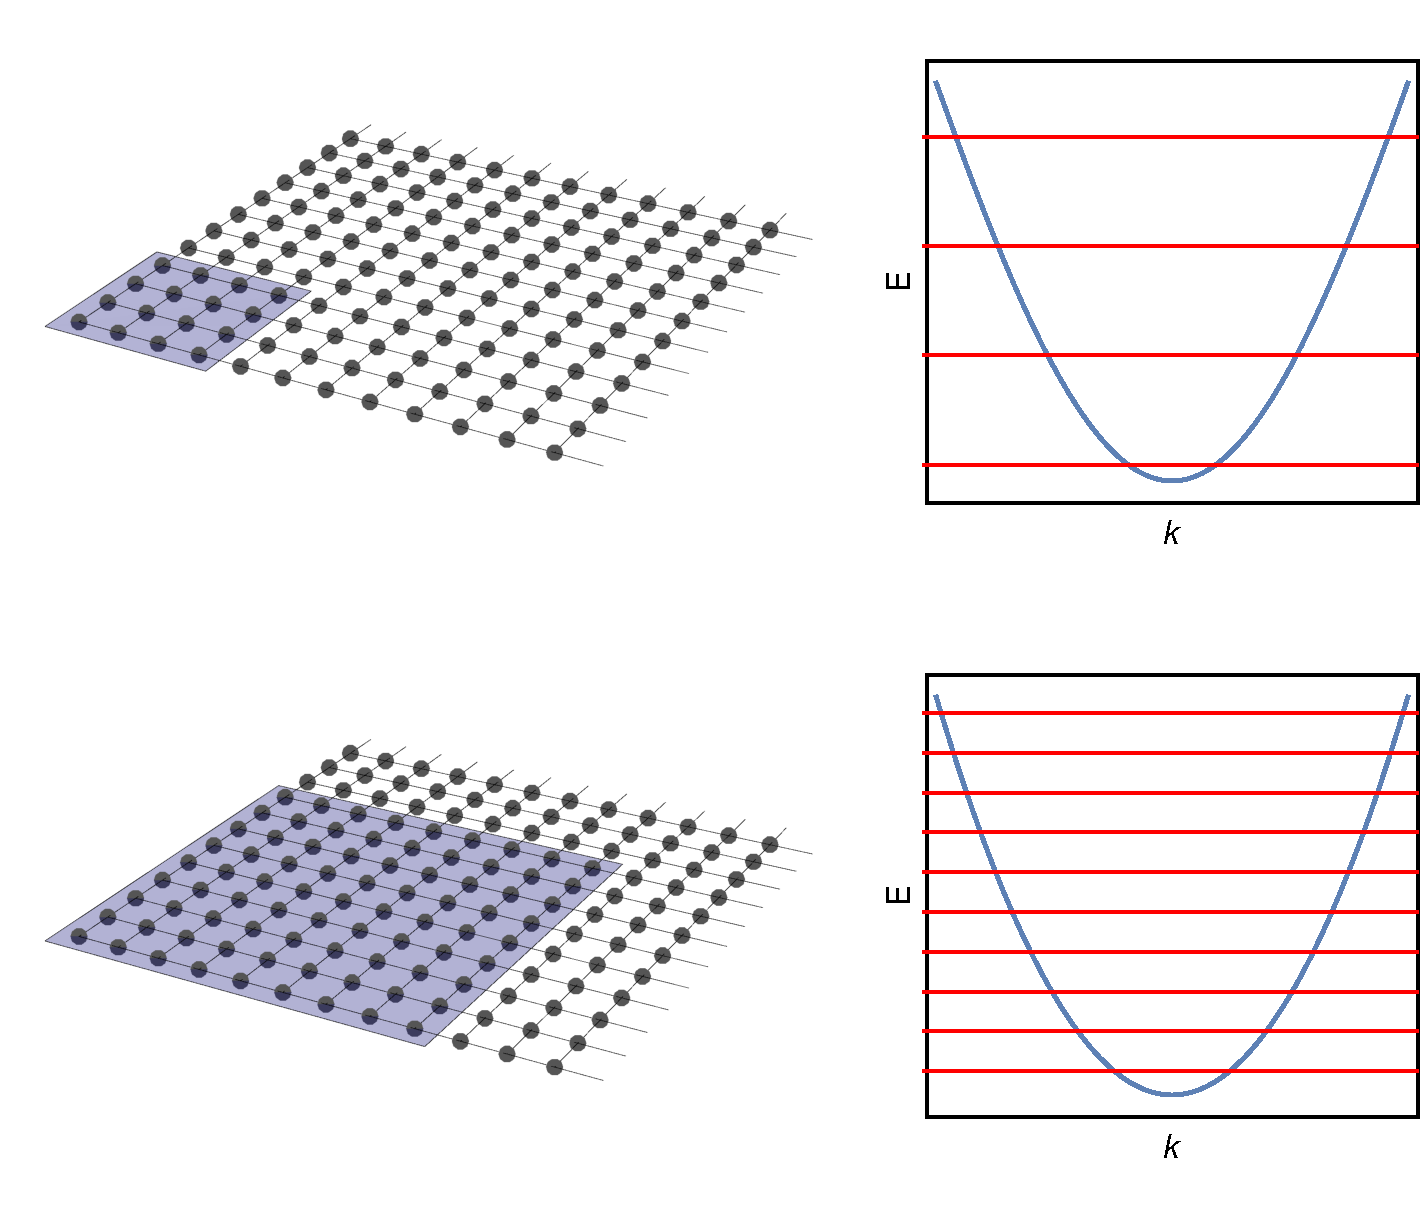
\includegraphics[width=3.1in]{test.pdf}
\caption{\label{bands-schematic}Schematic depiction of Landau-levels as the weak-field limit of Harper-Hofstadter bands near the minimum of a periodic potential. As the flux per plaquette is decreased, the elementary magnetic unit cell -- represented by the blue region of the lattice -- must increase in size to enclose the same number of flux quanta. In turn, the number of states in within each band decreases, and each band comprises states increasingly close to the minimum of the zero-field dispersion.}
\end{figure}

\section{Modified Harper-Hofstadter model}
In this section, we consider with additional next-nearest-neigbor (NNN) hopping amplitudes:
\begin{align}
\label{quartic-harper}
H_0 = &-t_1 \left(\widetilde{T}_1 + \widetilde{T}_1^{\dag} + \widetilde{T}_2 + \widetilde{T}_2^{\dag}\right)\nonumber\\ &- t_2 \left(\widetilde{T}_1^{2} + \widetilde{T}_1^{\dag 2} + \widetilde{T}_2^{2} + \widetilde{T}_2^{\dag 2}\right).
\end{align}
Note that this hamiltonian only contains straight-line lattice translations, and omits NNN hopping between opposite plaquette corners. 

%The hopping terms are depicted schematically in Fig. \ref{hoppings}. 

% \begin{figure}[thb]
% \centering
% 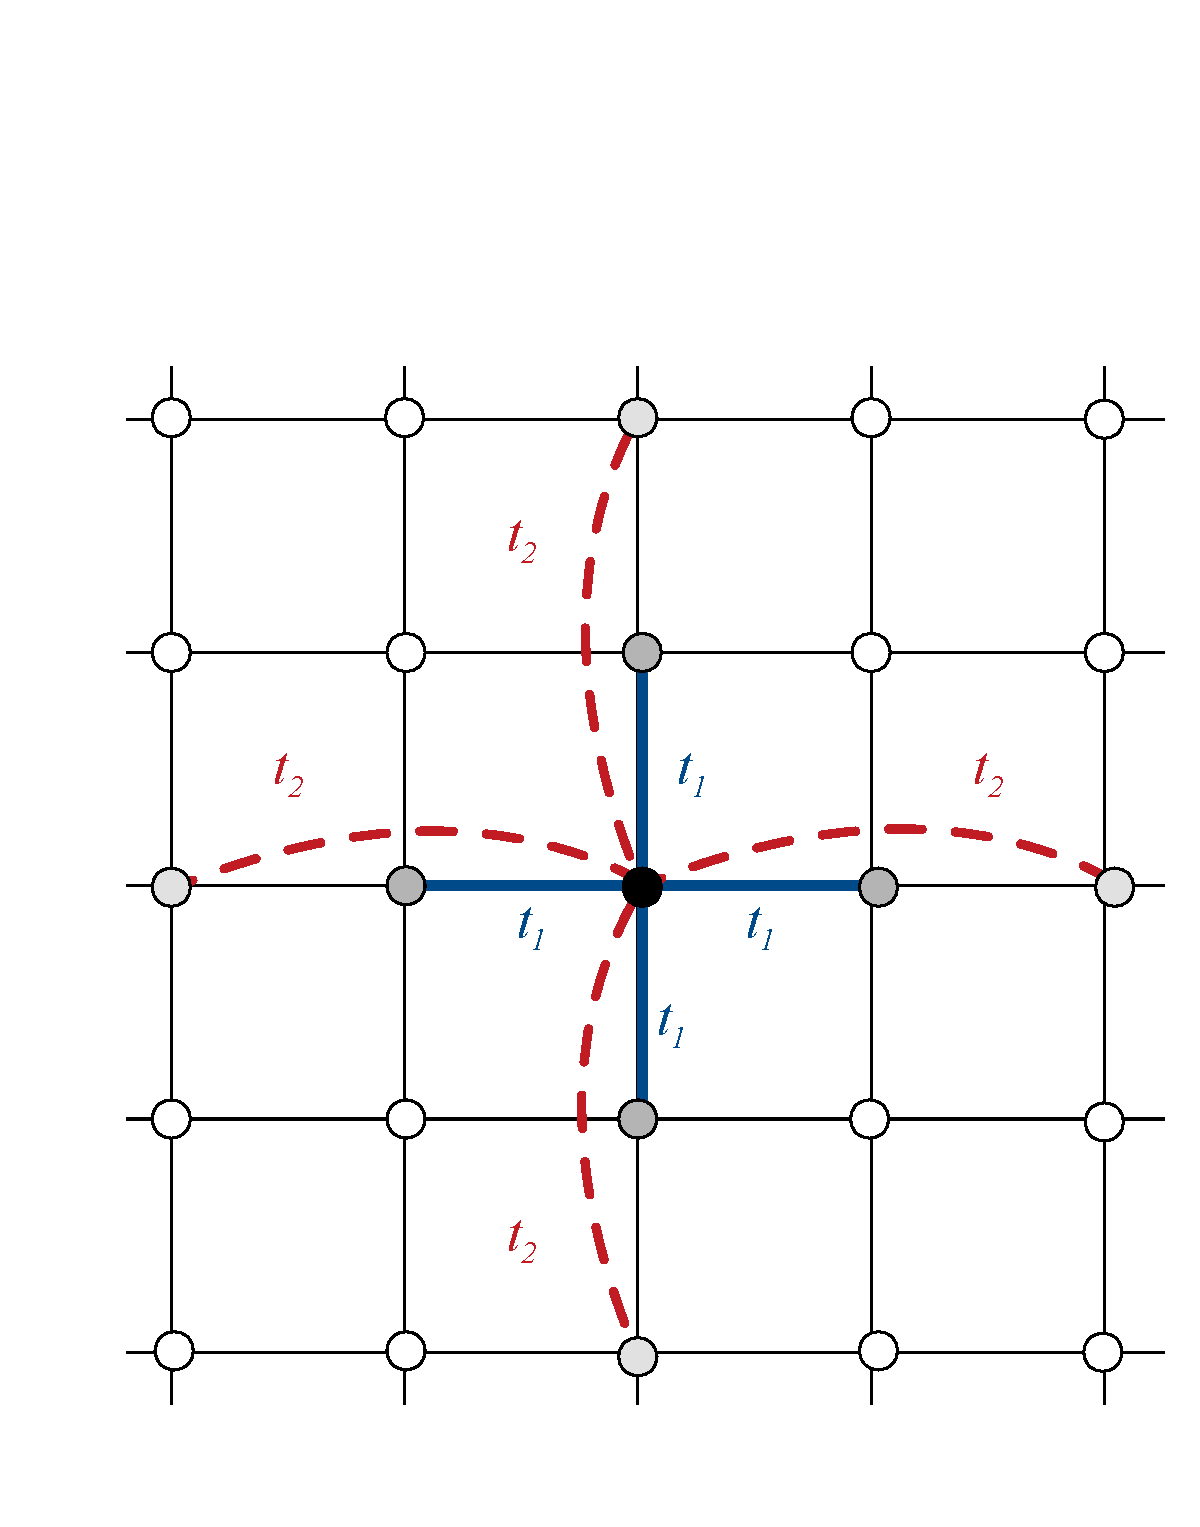
\includegraphics[width=1.5in]{quartic-hofstadter-hoppings-2.pdf}
% \caption{\label{hoppings} Nearest-neighbor (NN) and next-nearest-neighbor hopping terms included in the hamiltonian (\ref{quartic-harper}). For the fine-tuned model, we set $t_2 = -t_1/4$.}
% \end{figure}


% \begin{figure}[thb]
% \centering
% 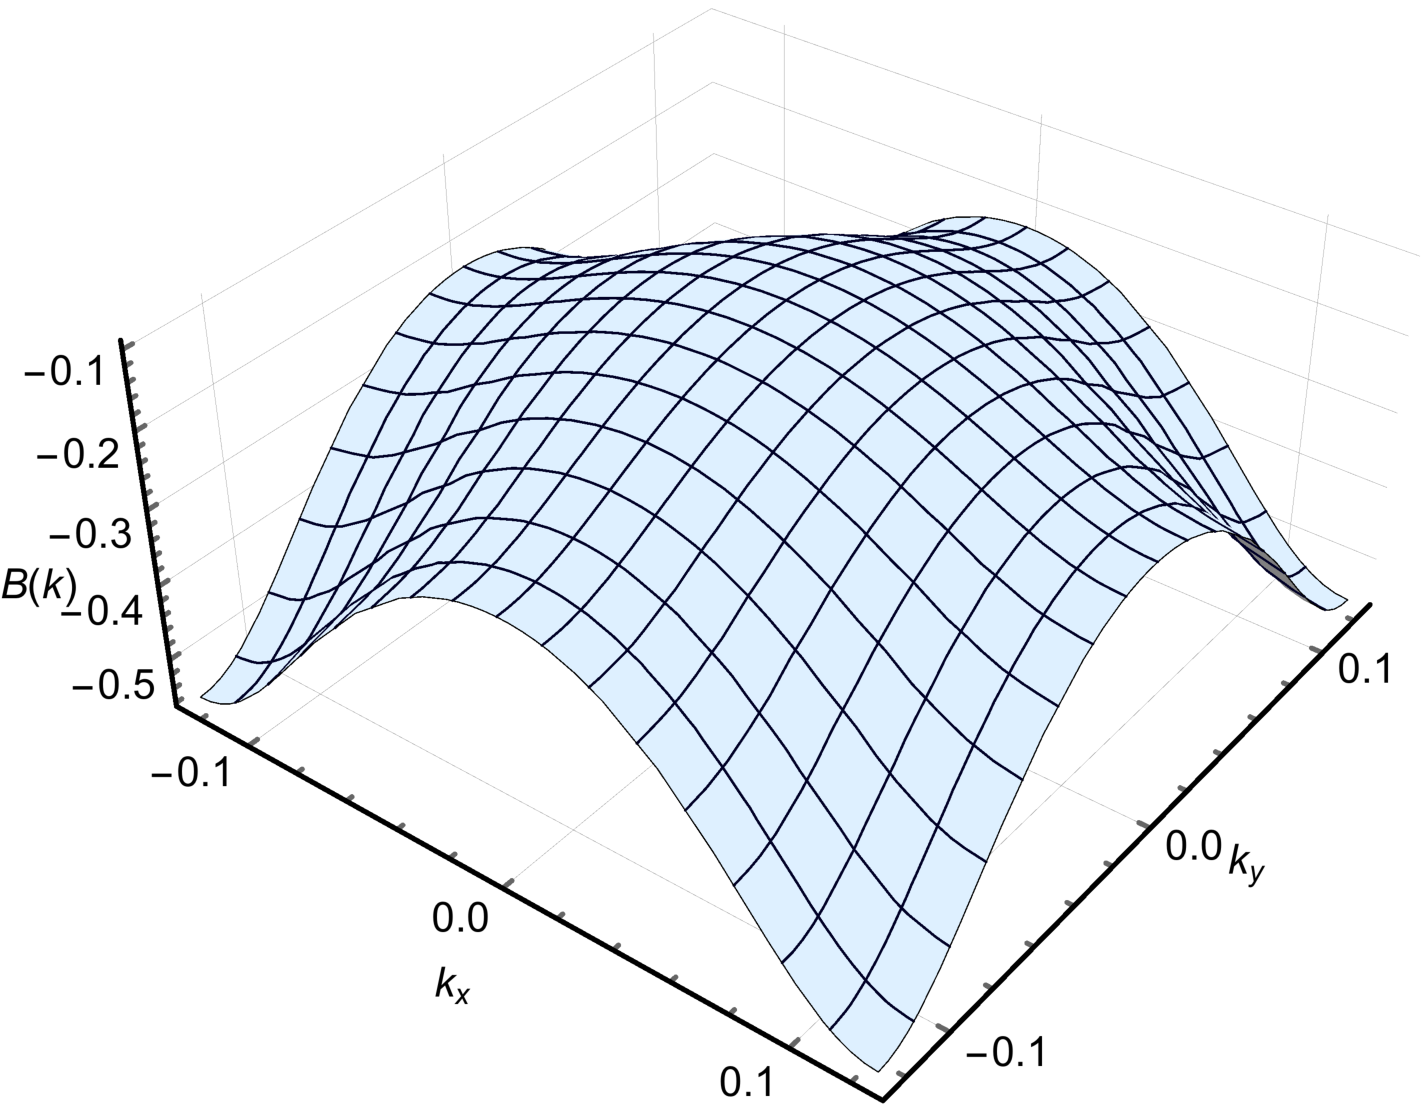
\includegraphics[width=3in]{hof-curvature-2.pdf}
% 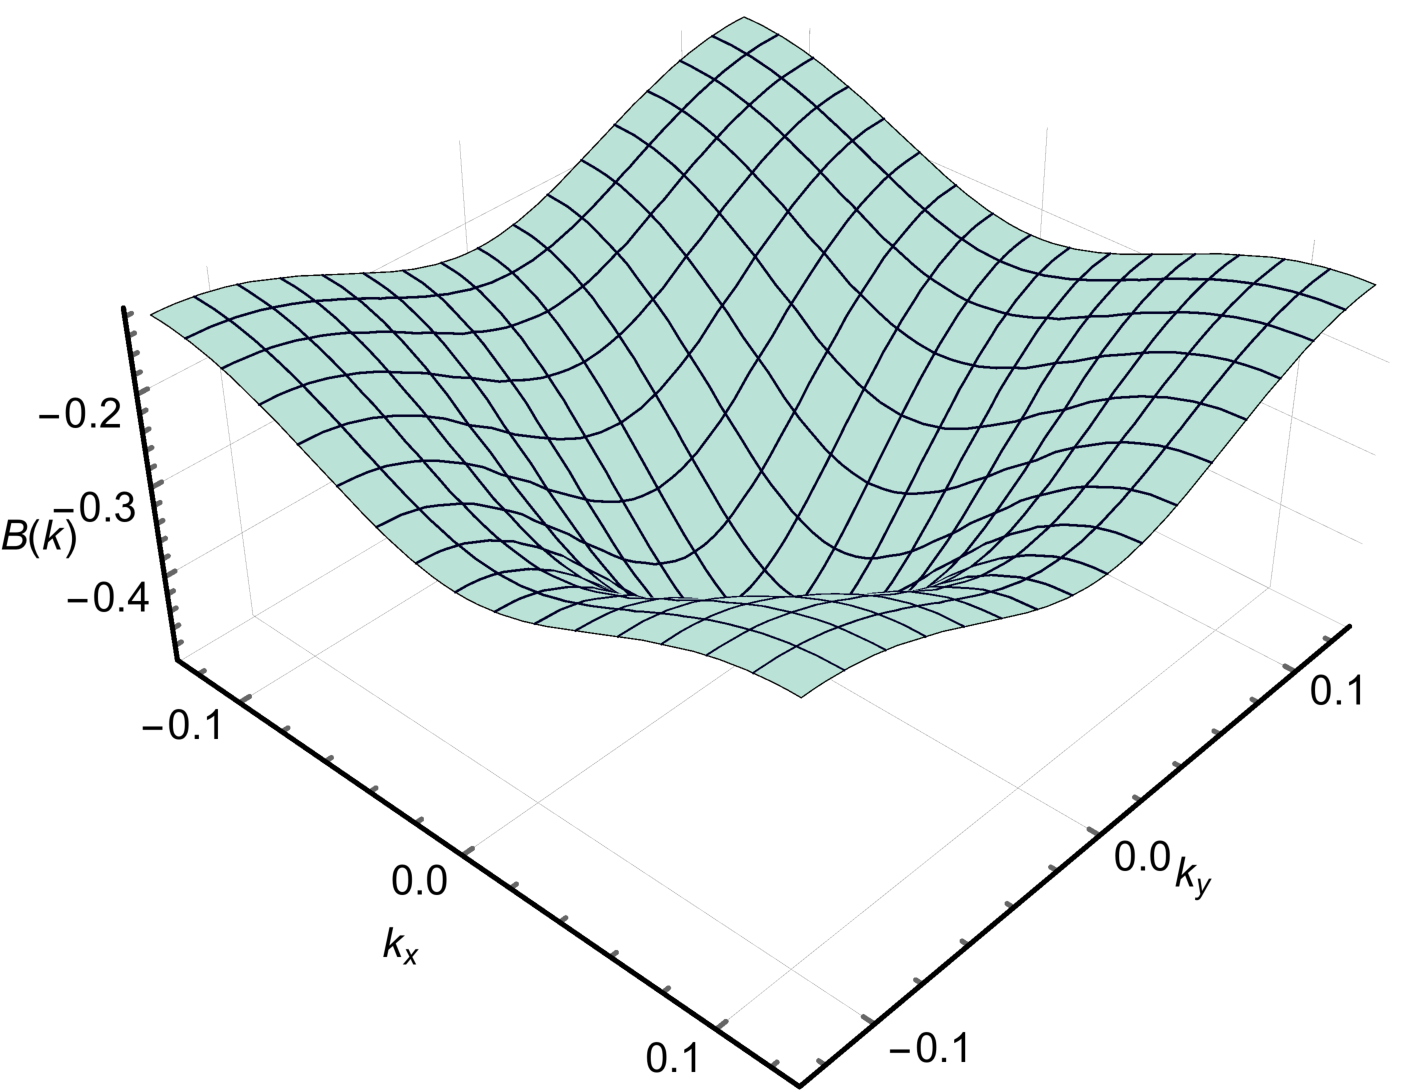
\includegraphics[width=3in]{quartic-curvature-2.pdf}
% \caption{\label{curv-fluctuations} Comparison of fluctuations in Berry curvature $B(\mathbf{k})$ over the magnetic Brillouin zone for the Hofstadter model (top) and the quartic model (\ref{quartic-harper}) (bottom) at the fine-tuned point $t_2 = -t_1/4$. The flux per plaquette in both cases is $\phi/\Phi_0 = 1/4$. The integral of $B(\mathbf{k})$ over the MBZ -- the Chern number -- has magnitude 1 for both bands.}
% \end{figure}

\begin{figure}[thb]
\centering
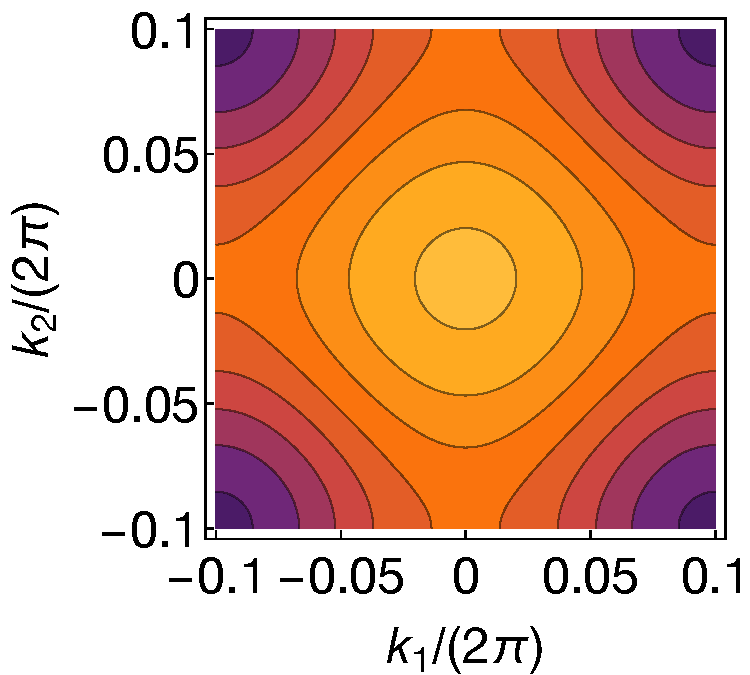
\includegraphics[width=1.4in]{curv-hof-n5.pdf}
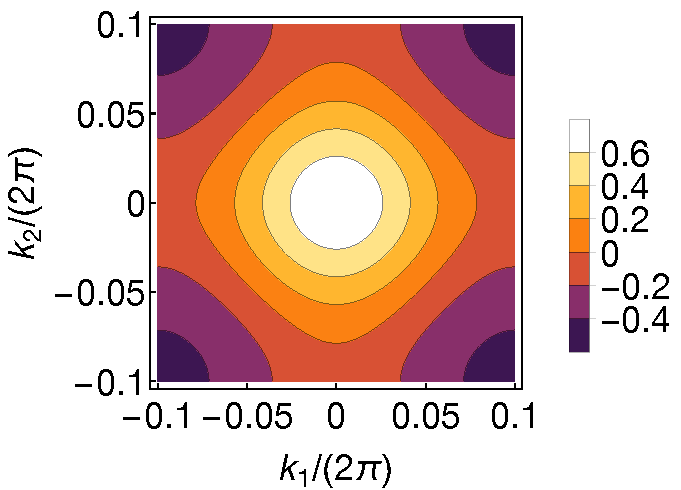
\includegraphics[width=1.75in]{curv-qrt-n5.pdf}
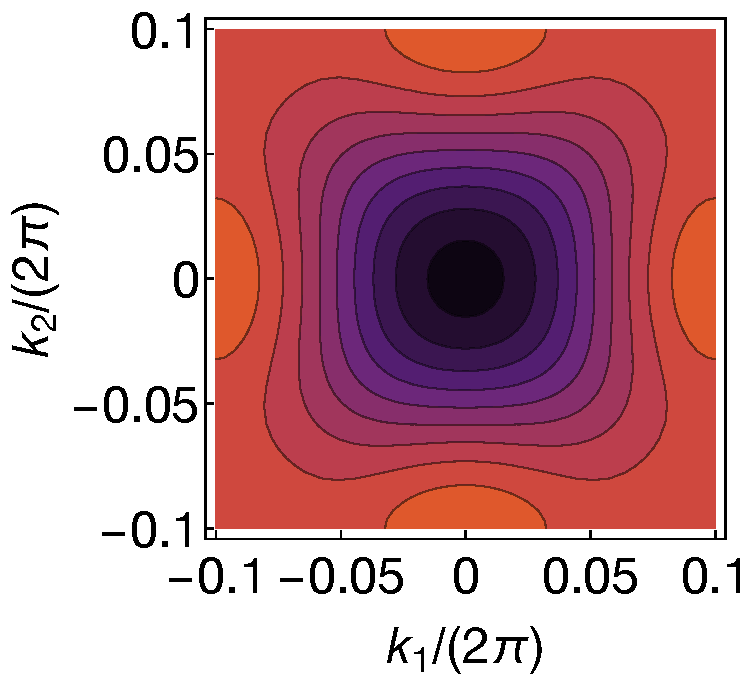
\includegraphics[width=1.4in]{norm-tr-hof-n5.pdf}
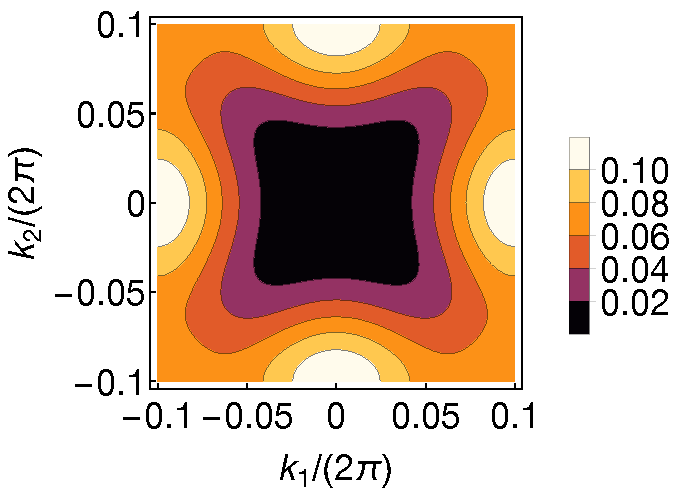
\includegraphics[width=1.75in]{norm-tr-qrt-n5.pdf}
\caption{Comparison of magnetic Brillouin zone geometry between Hofstadter (left) and quartic (right) models at flux per plaquette $\phi/\phi_0=1/5$. The top left panel shows the Berry curavture $B(\mathbf{k})$ for the Hofstadter model; the top right panel shows $B(\mathbf{k})$ for the quartic model. The bottom panels show the normalized trace inequality $\bar{T}(\mathbf{k})$ for these models.}
\end{figure}

As in Section \ref{landau-level-limit}, we write this in terms of the hermitian generators of lattice translations,
\begin{align*}
H_0 = &-2t_1\left(\cos(\Pi_1) + \cos(\Pi_2)\right)\\ &- 2t_2\left(\cos(2\Pi_1) + \cos(2\Pi_2)\right)
\end{align*}
Replacing the cosine terms by their Taylor expansion, the terms lowest-order in the momenta are 
\begin{align*}{}
H_0 = &-4 t_1 - 4 t_2 + (t_1 + 4t_2) \left(\Pi_1^2 + \Pi_2^2\right) \\
&- \left(\frac{t_1}{12} + \frac{4}{3}t_2\right) \left(\Pi_1^4 + \Pi_2^4\right) + \ldots
\end{align*}

If we make the particular choice of hopping amplitudes $t_2 = -t_1/4$, then the quadratic terms vanish exactly, and we are left with an effective hamiltonian that is quartic in the momenta to lowest order,
\begin{align}
\label{hamiltonian-quartic-effective}
H_{\text{eff}} = -3t_1 + \frac{t_1}{4} \left(\Pi_1^4 + \Pi_2^4\right).
\end{align}
Such negative hopping amplitudes can be realized in optical lattice experiments by periodic shaking of the lattice\cite{eckardt_colloquium_2017}. Unlike the Landau level hamiltonian, this hamiltonian does not have $SO(2)$ rotational symmetry, but it is symmetric under the square lattice isometry group $D_4$. It is somewhat interesting to plot the energy eigenvalues obtained from the Harper-type equation for this model as a function of $\phi = \hbar a^2/(e \ell^2)$ -- the analogue of the Hofstadter ``butterfly'' for this model\cite{hofstadter_energy_1976}. We display this in Fig. \ref{butterfly-plot}. In the Hofstadter model, where the bands appear approximately linear in $\phi$ near $\phi = 0$, the present model has bands that are roughly quadratic in $\phi$ in this region. We compute the Berry curvature and Chern number of these bands for $\varepsilon^2 = \frac{1}{N}$ and verify that they have Chern number $|c_1| = 1$.

\begin{figure}[thb]
\centering
\hspace{-0.25in}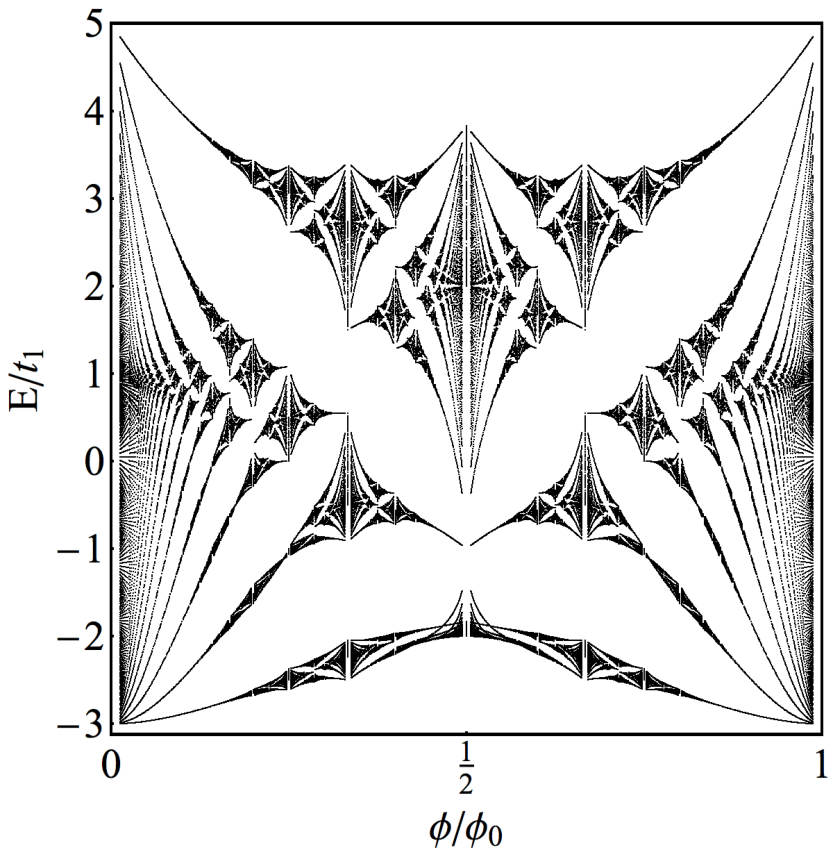
\includegraphics[width=3.0in]{q-butterfly-raster-1200.pdf}
\caption{\label{butterfly-plot} Energy eigenvalues of the lattice Harper-Hofstadter hamiltonian (\ref{quartic-harper}) with $t_1 = 1$, $t_2 = -1/4$ as a function of magnetic flux per elementary lattice plaquette $\phi/\phi_0 = \varepsilon^2/(2\pi) = P/Q$.}
\end{figure}

The particular quartic momentum operator in (\ref{hamiltonian-quartic-effective}) can be written
\begin{align*}
\Pi_1^4 + \Pi_2^4 = \left(\Pi_1^2 + \Pi_2^2\right)^2 - \left(\Pi_1^2\Pi_2^2 + \Pi_2^2\Pi_1^2\right),
\end{align*}
that is, as the square of the Landau-level hamiltonian plus a term that explicitly breaks the rotational symmetry.

As in the Landau level problem, we study the spectrum of this model by introducing Fock operators $a$, $a^{\dag}$ corresponding to the cyclotron momenta $\Pi_a$. For example, we choose the operators
\begin{align*}
a &= \frac{1}{\sqrt{2}\varepsilon}\left(\Pi_1 - i\Pi_2\right),\\
a^{\dag} &= \frac{1}{\sqrt{2}\varepsilon}\left(\Pi_1 + i\Pi_2\right).
\end{align*}
In terms of these operators,
\begin{align*}
\left(\Pi_1^2 + \Pi_2^2\right)^2 &= 4\left(a^{\dag}a + \frac{1}{2}\right)^2, \\
\Pi_1^2\Pi_2^2 + \Pi_2^2\Pi_1^2 &= -\frac{1}{2}\left(a^4 + a^{\dag\,4}\right) + \left(a^{\dag}a + \frac{1}{2}\right)^2 - \frac{3}{4},
\end{align*}
and the effective hamiltonian is
\begin{align}
\label{effective-fock-hamiltonian}
H_{\text{eff}} = \frac{t_1\varepsilon^4}{8}\left[a^4 + a^{\dag 4} + 6\left(a^{\dag}a + \frac{1}{2}\right)^2 + \frac{3}{2}\right].
\end{align}

We numerically approximate this hamiltonian by working in a basis of number eiegenstates $\ket{n}$ staisfying $a^{\dag}a{\ket{n}}=n{\ket{n}}$ and truncating to a finite-dimensional subspace. This gives estimates for the cyclotron energies and overlaps with the Landau level states. We find good agreement between this continuum approximation truncated to $n \leq 1000$ and exact numerical energy levels of lattice hamiltonian for small $\varepsilon$. The first two nonzero overlaps of the ground state $\ket{\tilde{0}}$ of the hamiltonian (\ref{effective-fock-hamiltonian}) with the Landau level states are $\braket{\tilde{0}}{0}\approx0.9991$, $\braket{\tilde{0}}{4}\approx-0.0422$. In terms of Fock operators, the trace inequality takes the particularly simple form $\expval{T} = 2\expval{a^{\dag}a}$\cite{bauer_quantum_2016}. Calculating this in the truncated Landau level basis, we find $\expval{T} \approx0.0143$, in good agreement with the value found from intergrating the lattice $T(\mathbf{k})$ over the MBZ, $\expval{T} \approx 0.0145$.

We also study the spectrum of cyclotron orbits of this hamiltonian semiclassically by applying the Bohr-Sommerfeld quantization condition. In our notation this is
\begin{align*}
\oint\limits_{H=E_n} \Pi_1\, d\Pi_2 = 2\pi n,
\end{align*}
with the integral taken over a closed curve of constant energy in classical phase space. From this condition we find
\begin{align*}
E_n \sim n^2\phi^2, 
\end{align*}
in agreement both with the numerically-obtained, approximate spacing of the cyclotron levels, and with the quadratic dependence of $E$ on $\phi$ observed in the butterfly plot, Fig. \ref{butterfly-plot}.

% Geometric stability considerations\cite{jackson_geometric_2015} then suggest that the trace inequality $\expval{T}$ should provide information about the size of the many-body gap.

\subsection{Deviations from fine-tuning}
We now consider small perturbations away from the fine-tuned case $t_2 = -t_1/4$ by seting $t_2 = \left(-\frac{1}{4} + \delta\right)t_1$. In this case, instead of (\ref{hamiltonian-quartic-effective}) above, we have an effective hamiltonian with a quadratic term, ,
\begin{align}
\label{delta-hamiltonian}
H_{\text{eff}} = t_1 \left[\left(\frac{1}{4}-\frac{4\delta}{3}\right)\left(\Pi_1^4 + \Pi_2^4\right) + 4\delta \left(\Pi_1^2 + \Pi_2^2\right)\right].
\end{align}
For a fixed $\delta$, we may decrease the external magnetic flux density $B$, and hence $\varepsilon$, such that the quadratic term dominates, and our Chern bands are effectively Landau levels. However, for a fixed $\varepsilon$, $\delta$ may be small enough that the quadratic term can be treated as a perturbation to the quartic term. A weak upper bound on the range of the small $\delta$ regime is given by stipulating that the relative strength of the quadratic term 
\begin{align*}
\frac{1}{\varepsilon^2}\frac{48\delta}{3-16\delta} < 1.
\end{align*}
While we have introduced $\delta$ to parameterize perturbations from our fine-tuned model, we could also view $\delta$ as a tunable parameter in its own right. In particular, varying $\delta$ between $0$ and $1/4$ interpolates between our quartic model ($\delta=0$) and the Hofstadter model ($\delta=1/4$). We numerically calculate the value of the trace inequality of this model $\expval{T}$ for a few $\delta$ in this interval, and plot the results in Fig. (\ref{trace-delta-plot}). We attribute the minima appearing in Fig. (\ref{trace-delta-plot}) in the region between the to the vanishing of the quartic term in the hamiltonian at these points.

\begin{figure}[thb]
\centering
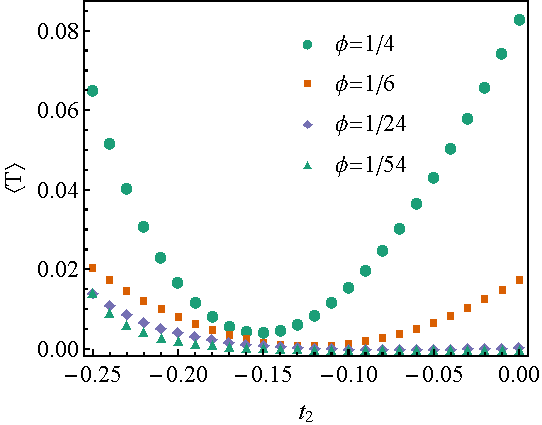
\includegraphics[width=3.0in]{trace-delta-plot-new.pdf}
\caption{\label{trace-delta-plot}Magnetic Brillouin zone-averaged trace inequality $\expval{T}$ for the lowest-lying band of (\ref{quartic-harper}) as a function of $\delta$.}
\end{figure}


\subsection{Many-body gap from numerical exact diagonalization}
The bands of our weak-field lattice hamiltonian correspond to cyclotron orbits that are distinct from Landau levels. However, we still expect that fractionally filling these bands with interacting particles will lead to FQH phases. To verify this, we numerically diagonalize a two-body, nearest-neighbor interaction hamiltonian projected to these bands. This interaction hamiltonian is known to stabilize the Laughlin state at $\nu = 1/3$ in the Hofstadter model. We carry out our numerical diagonalization on a torus, and verify that the many-body ground states have the appropriate topological degeneracy for a Laughlin fluid on a torus. We also verify that under three-fold insertion of $2\pi$ flux, the degenerate ground states flow into one another and do not mix with excited states.

For both the Hofstadter model and our quartic model, variations of the energy dispersion, Berry curvature, and Fubini-Study metric over the MBZ decrease exponentially as $\phi$ decreases\cite{Harper:2014vi,bauer_quantum_2016}. However, the BZ-averaged band-geometric inequalities (\ref{band-geom-ineq}) vanish polynomially. That is, even when fluctuations in band geometry are negligibly small, these inequalities provide a measure of deviations from Landau level behavior. Geometric stability considerations \cite{jackson_geometric_2015} suggest that the size of the many-body gap should decrease as the trace inequality varies from the LLL value $\expval{T}=0$.


\begin{figure*}[thb]
\centering
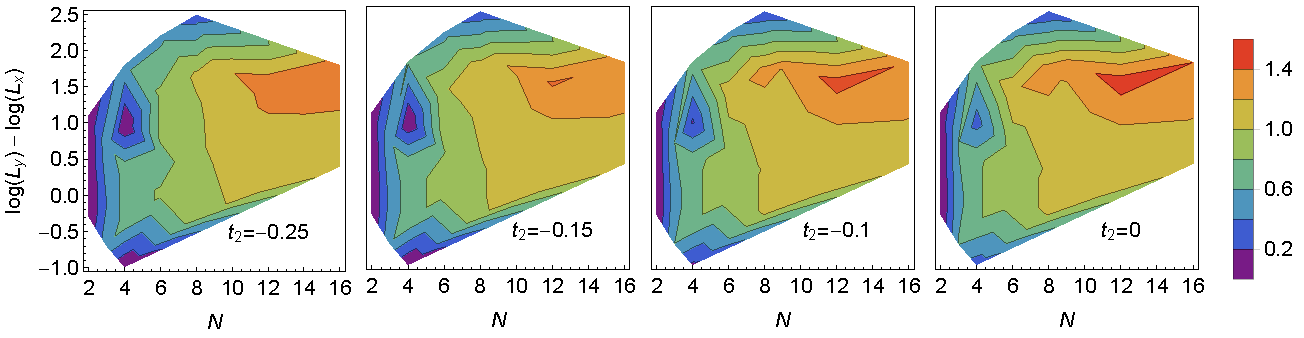
\includegraphics[width=6.3in]{gap-grid-2.pdf}
\caption{Many-body gap of a $\nu=1/3$ Laughlin state of $N_p=8$ fermions in the lowest band of the modified Hofstadter model for $\phi = \phi_0/N$ and multiple values of $t_2$. The horizontal axis in each plot is the reciprocal $N$ of the flux per plaquette, while the vertical axis $\log(L_y/L_x)$ measures the overall anisotropy of the system with $L_x$ ($L_y$) the total number of lattice sites in the $x$ ($y$) direction. When $\log(L_y/L_x)=0$, the system is perfectly isotropic. }
\end{figure*}


\begin{figure}[thb]
\centering
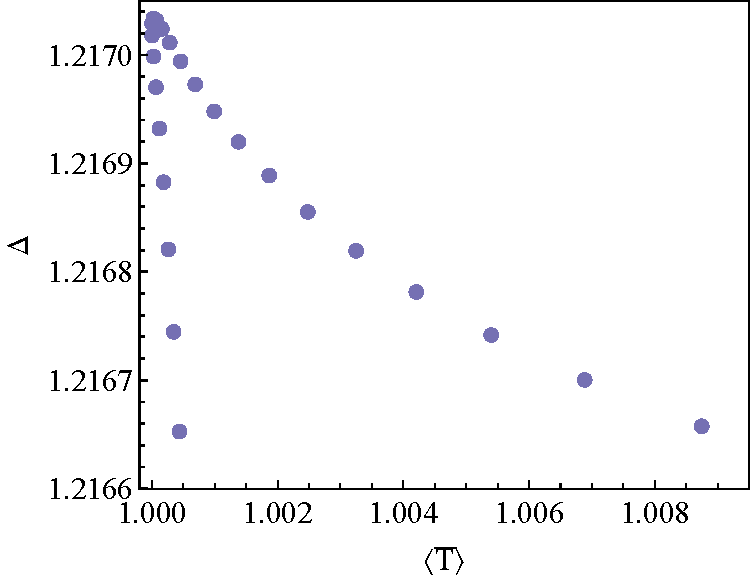
\includegraphics[width=3.0in]{gap-v-trace-delta.pdf}
\caption{\label{gap-v-trace-delta-plot}Many-body gap of $N_p=8$ interacting fermions at $\nu=1/3$ filling in the lowest band of the quartic model (\ref{quartic-harper}). In this plot, $\phi/\phi_0=1/24$, and the fermions interact via a repulsive next-nearest-neighbor potential. Each point correspond to a different value of $\delta$. This plot shows two different regimes with different dependence $\Delta$ on $\expval{T}$. The more slowly decreasing branch of the plot corresponds to $\delta < 0.16$, and the other branch to $\delta > 0.16$. The largest gap is observed where the two branches converge, at $\delta = 0.16$.}
\end{figure}

% Consider just the quadratic part of this hamiltonian,
% \begin{align*}
% H_0 = h_{ab}\Pi_a \Pi_b
% \end{align*} We would like to choose Fock operators such that $H_0 = \frac{\omega}{2}\left(a^{\dag}a + aa^{\dag}\right).$ One way to implement this map would be to first perform a coordinate transformation on the momentum phase space that diagonalizes the effective mass tensor $h_{ab}$, then introduce Fock operators in, e.g. the Landau gauge in terms of the new momenta. A second way to do this is to forgoe the coordinate transformation and explicitly choose Fock operators that bring $H_0$ into this form.

% A choice of Fock operators is equivalent to a choice of positive complex structure on $\mathbf{R}^2$ compatible with the symplectic form on $\mathbf{R}^2$. A generic choice of such a complex structure is equivalent to a choice of $\tau \in \mathbf{H}$, with $\mathbf{H} = \left\{\tau \in \mathbf{C}, \text{Im}\,\tau >0\right\}$ the complex upper half-plane, and yields Fock operators
% \begin{align*}
% a = \frac{1}{\sqrt{2\tau_2}\epsilon}\left(\Pi_1 - \tau\Pi_2\right)\\
% a^{\dag} = \frac{1}{\sqrt{2\tau_2}\epsilon}\left(\Pi - \tau^{\ast}\Pi_2\right).
% \end{align*}

% In order to put our hamiltonian to take the form $H_0 = \omega\left(a^{\dag}a + aa^{\dag}\right)/2$, we choose
% \begin{align*}
% \tau = \frac{1}{h_{11}}\left(\sqrt{|h|} - i h_{12}\right).
% \end{align*}
% where $|h| = \text{det}\,h = \omega^2/(4\varepsilon^4).$

\section{Conclusion}
In conclusion, we have constructed a Harper-Hofstadter model with cyclotron orbits that are distinct from Landau levels in the continuum limit. This provides a regime in which to study the quantum Hall effect that is distinct from both the Landau level 2DEG and FCI models. 

While we have focused on a particular choice of hopping amplitudes, by including longer-range hoppings and tuning them appropriately, one may obtain arbitrary inversion-symmetric dispersion relations. In particular, we could arrage our hamiltonian so that both quadratic and quartic terms vanish, leaving only a sextic term -- and so on. Put slightly differently, the construction that we have outlined here may in principle be used to construct infinite families of lattice hamiltonians that do not have Landau levels as their continuum cyclotron orbits.

One drawback of our numerical approach is that we diagonalize the many-body interaction hamiltonian on a lattice. While this is not a problem in the FCI regime, it may obscure the physics in the continuum regime, for example by gapping potential symmetry-breaking Goldstone modes that would be gapless in the continuum. Using DMRG or other numerical techniques that do not rely directly on a tight-binding description may rememedy this. Another drawback of constructing continuum bands from lattice model is that the continuum models inherit non-generic point-group symmetries from the lattice geometry, so that we do not obtain fully generic bands in this way.

\begin{acknowledgments}
The authors thank Tom Jackson for collaboration on related work and for his band geometry code. We also thank authors of the DiagHam package, which was used in this work.

\end{acknowledgments}
\bibliographystyle{apsrev4-1}
\bibliography{landau-orbits}
%\bibliography{quartic-zotero/quartic-zotero}

\clearpage
\appendix
\section{Weak-field effective hamiltonian for Hofstadter model $C_4$ symmetric NNN hopping}
For completeness, we reproduce here the  Hofstadter model with all next-nearest-neighbor (NNN) hopping terms that respect $C_4$ symmetry, including the hopping diagonally across a plaquette. The tight-binding hamiltonian is
\begin{align*}
H_0 = &-t_1 \left(\widetilde{T}_1 + \widetilde{T}_2\right)\nonumber - t_2 \left(\widetilde{T}_1^{2} + \widetilde{T}_2^{2}\right)\\ &- t_3 \left(\widetilde{T}_1\widetilde{T}_2 + \widetilde{T}_2 \widetilde{T}_1\right) + \text{h.c.}
\end{align*}

We can write this in terms of the generators $\Pi_a$ as
\begin{align*}
H_0 = &-2t_1 \left[\cos\left(\Pi_1\right) + \cos\left(\Pi_2\right)\right]\\ &-2t_2 \left[\cos\left(2\Pi_1\right)+\cos\left(2\Pi_2\right)\right]\\ &- 4t_3 \cosh\left(\frac{\epsilon^2}{2}\right)\cos\left(\Pi_1 + \Pi_2\right).
\end{align*}
The factor of $\cosh(\epsilon^2/2)$ is non-universal and results from our ordering prescription.

Expanding to quartic order, we obtain the low-$\epsilon$ effective hamiltonian
\begin{align*}
H_{\text{eff}} = h_{ab}\Pi_a \Pi_b + \lambda_{abcd} \Pi_a \Pi_b \Pi_c \Pi_d 
\end{align*}

with coefficients

\begin{align*}
h_{11} = h_{22} &= t_1 + 4t_2 + 2t_3,\\
h_{12} &= 2t_3,
\end{align*}
and 
% \begin{align*}
% \lambda_{1111} &= \lambda_{2222} = -\frac{1}{3}\left(t_1/4 + 4t_2 + t_3/2\right)
% \lambda_{1112}  &= \lambda_{1222} = -t_3/3\\
% \lambda_{1122} &= -t_3/2
% \begin{align*}
\begin{align*}
\lambda_{1111} = \lambda_{2222} &= -\frac{1}{3}\left(\frac{t_1}{4} + 4t_2 + \frac{t_3}{2} \right),\\
\lambda_{1112}  = \lambda_{1222} &= -t_3/3,\\
\lambda_{1122} &= -t_3/2.
\end{align*}




% \section{Quartic hamiltonian effective hamiltonian for $C_4$ symmetric NNN hoppings.}
% In this section, we consider the Hofstadter model with all next-nearest-neighbor (NNN) hopping terms -- including the hopping diagonally across a plaquette and find the effective quartic hamiltonian. The hoppings are selected to preserve the underlying $C_4$ symmetry of the lattice. Specifically, we choose 
% \begin{align*}
% H_0 = &-t_1 \left(\widetilde{T}_1 + \widetilde{T}_2\right)\nonumber - t_2 \left(\widetilde{T}_1^{2} + \widetilde{T}_2^{2}\right)\\ &- t_3 \left(\widetilde{T}_1\widetilde{T}_2 + \widetilde{T}_2 \widetilde{T}_1\right) + \text{h.c.}
% \end{align*}

% We can write this in terms of the generators $\Pi_a$ as
% \begin{align*}
% H_0 = &-2t_1 \left[\cos\left(\Pi_1\right) + \cos\left(\Pi_2\right)\right]\\ &-2t_2 \left[\cos\left(2\Pi_1\right)+\cos\left(2\Pi_2\right)\right]\\ &- 4t_3 \cosh\left(\frac{\epsilon^2}{2}\right)\cos\left(\Pi_1 + \Pi_2\right).
% \end{align*}

% Expanding to quartic order, we obtain the low-$\epsilon$ effective hamiltonian
% \begin{align*}
% H_{\text{eff}} = h_{ab}\Pi_a \Pi_b + \lambda_{abcd} \Pi_a \Pi_b \Pi_c \Pi_d 
% \end{align*}

% with coefficients

% \begin{align*}
% h_{11} = h_{22} &= t_1 + 4t_2 + 2t_3,\\
% h_{12} &= 2t_3,
% \end{align*}
% and 
% % \begin{align*}
% % \lambda_{1111} &= \lambda_{2222} = -\frac{1}{3}\left(t_1/4 + 4t_2 + t_3/2\right)
% % \lambda_{1112}  &= \lambda_{1222} = -t_3/3\\
% % \lambda_{1122} &= -t_3/2
% % \begin{align*}
% \begin{align*}
% \lambda_{1111} = \lambda_{2222} &= -\frac{1}{3}\left(\frac{t_1}{4} + 4t_2 + \frac{t_3}{2} \right),\\
% \lambda_{1112}  = \lambda_{1222} &= -t_3/3,\\
% \lambda_{1122} &= -t_3/2.
% \end{align*}


\end{document}


